\documentclass{beamer}

\mode<presentation> {
\usetheme{Singapore}
\setbeamercovered{transparent}

%\setbeamertemplate{footline} % To remove the footer line in all slides uncomment this line
%\setbeamertemplate{footline}[page number] % To replace the footer line in all slides with a simple slide count uncomment this line
%\setbeamertemplate{navigation symbols}{} % To remove the navigation symbols from the bottom of all slides uncomment this line
}

% \usepackage{ctex}
\usepackage{fontawesome}
\usepackage{graphicx} 
\usepackage{booktabs} 
\usepackage{xcolor}
\usepackage{calc}
\usepackage{amsmath}

\setbeamertemplate{caption}[numbered]

% \makeatletter
% \setbeamertemplate{frametitle}{
%     \ifbeamercolorempty[bg]{frametitle}{}{\nointerlineskip}%
%     \@tempdima=\textwidth%
%     \advance\@tempdima by\beamer@leftmargin%
%     \advance\@tempdima by\beamer@rightmargin%
%     \vspace*{1cm} %%%%%%%%%%%%% For example insert shift to right
%     \begin{beamercolorbox}[sep=0.3cm,center,wd=\the\@tempdima]{frametitle}
%         \usebeamerfont{frametitle}%
%         \vbox{}\vskip-1ex%
%         \if@tempswa\else\csname beamer@ftecenter\endcsname\fi%
%         {%
%             \ifx\insertframesubtitle\@empty%
%             \else%
%             {\usebeamerfont{framesubtitle}\usebeamercolor[fg]{framesubtitle}\insertframesubtitle\strut\par}%
%             \fi
%         }%
%         \vskip-1ex%
%         \if@tempswa\else\vskip-.3cm\fi% set inside beamercolorbox... evil here...
%     \end{beamercolorbox}%
% }
% \makeatother

\newcommand{\vect}[1]{\boldsymbol{#1}}
\newcommand{\matr}[1]{\mathbf{#1}}
\newcommand{\lnn}[1]{
  \ln\left(#1\right)
}

\newlength\dlf
\newcommand\alignedbox[2]{
  % #1 = before alignment
  % #2 = after alignment
  &
  \begingroup
  \settowidth\dlf{$\displaystyle #1$}
  \addtolength\dlf{\fboxsep+\fboxrule}
  \hspace{-\dlf}
  \fcolorbox{red}{yellow}{$\displaystyle #1 #2$}
  \endgroup
}

% \pgfdeclareimage[height=0.7cm]{company-logo}{img/realtek.png}
% \logo{\pgfuseimage{company-logo}}

\author{\huge{Tzu-Chun, Oscar, Hsu}} 
\institute[National Yang Ming Chiao Tung University (NYCU)] 
{
    \normalsize{
        Institute of Computer Science and Engineering, \\
        National Yang Ming Chiao Tung University (NYCU)} \\~\\
    \scriptsize{
        \href{tel:+886-987605719}{ \raisebox{-0.1\height}\faPhone\ \underline{+886-987605719} ~} 
        \href{mailto:vm3y3rmp40719@gmail.com}{\raisebox{-0.2\height}\faEnvelope\  \underline{vm3y3rmp40719@gmail.com}} \\~\\
        \href{https://www.linkedin.com/in/tzu-chun-hsu-ab4b3b188/}{\raisebox{-0.2\height}\faLinkedinSquare\ \underline{tzu-chun-hsu-ab4b3b188} ~}
        \href{https://github.com/Oscarshu0719}{\raisebox{-0.2\height}\faGithub\ \underline{Oscarshu0719}}
    }
}
\date{November 21, 2024} 

\begin{document}

\begin{frame}
\titlepage % Print the title page as the first slide
\end{frame}

% \begin{frame}
% \frametitle{Table of contents} 
% \tableofcontents 
% \end{frame}

%----------------------------------------------------------------------------------------
%	EDUCATION SLIDES
%----------------------------------------------------------------------------------------

\section{Education}
\begin{frame}
    \frametitle{Education}
    \begin{block}{Zhejiang University} % #47 QS 2025.
        Bachelor of Engineering in Computer Science and Technology\\
        Hangzhou, China \hfill 09 2016 – 07 2020
    \end{block}
    \begin{block}{National Yang Ming Chiao Tung University}
        Master of Science in Computer Science and Engineering\\
        Hsinchu, Taiwan \hfill 09 2022 – 01 2025 (Expected)
    \end{block}
\end{frame}

%----------------------------------------------------------------------------------------
%	PROJECTS SLIDES
%----------------------------------------------------------------------------------------

\section{Projects}
\begin{frame}
    \frametitle{Projects}
    \begin{block}{\href{https://docs.google.com/presentation/d/1ge2It3UsAvTwpAk-9LUnmiz7dRqJnpFX/edit?usp=sharing&ouid=101248488395326982475&rtpof=true&sd=true}{1. Chord learning and adversarial framework for symbolic music generation}}
        \begin{itemize}
            \item Proposed a chord learning framework for multi-track symbolic music generation based on VAE and GAN.
            \item Introduced WGAN-GP to solve mode collapse and vanishing gradient problem.
        \end{itemize}

        \begin{figure}[H]
            \centering
            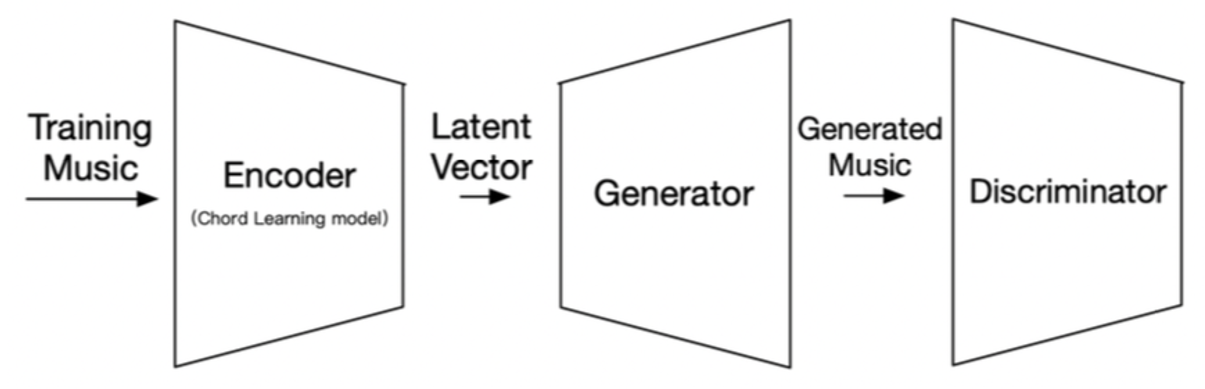
\includegraphics[scale=0.4]{img/srtp-arch.png}
        \end{figure}
    \end{block}
\end{frame}

\begin{frame}
    \frametitle{Projects}
    \begin{block}{\href{https://drive.google.com/file/d/1QqgPoRGhaSeS0QWrjnR8mxhvV_onwZ5y/view?usp=drive_link}{2. (Bachelor's Thesis) Voice Conversion Based on Generative Adversarial Networks}}
        \begin{itemize}
            \item Improved StarGAN-VC2 based on multi-speaker non-parallel corpus.
            \item Introduced WGAN-div, AdaIN layer, and neural vocoder, WaveGlow, for better results.
        \end{itemize}

        \begin{figure}[H]
            \centering
            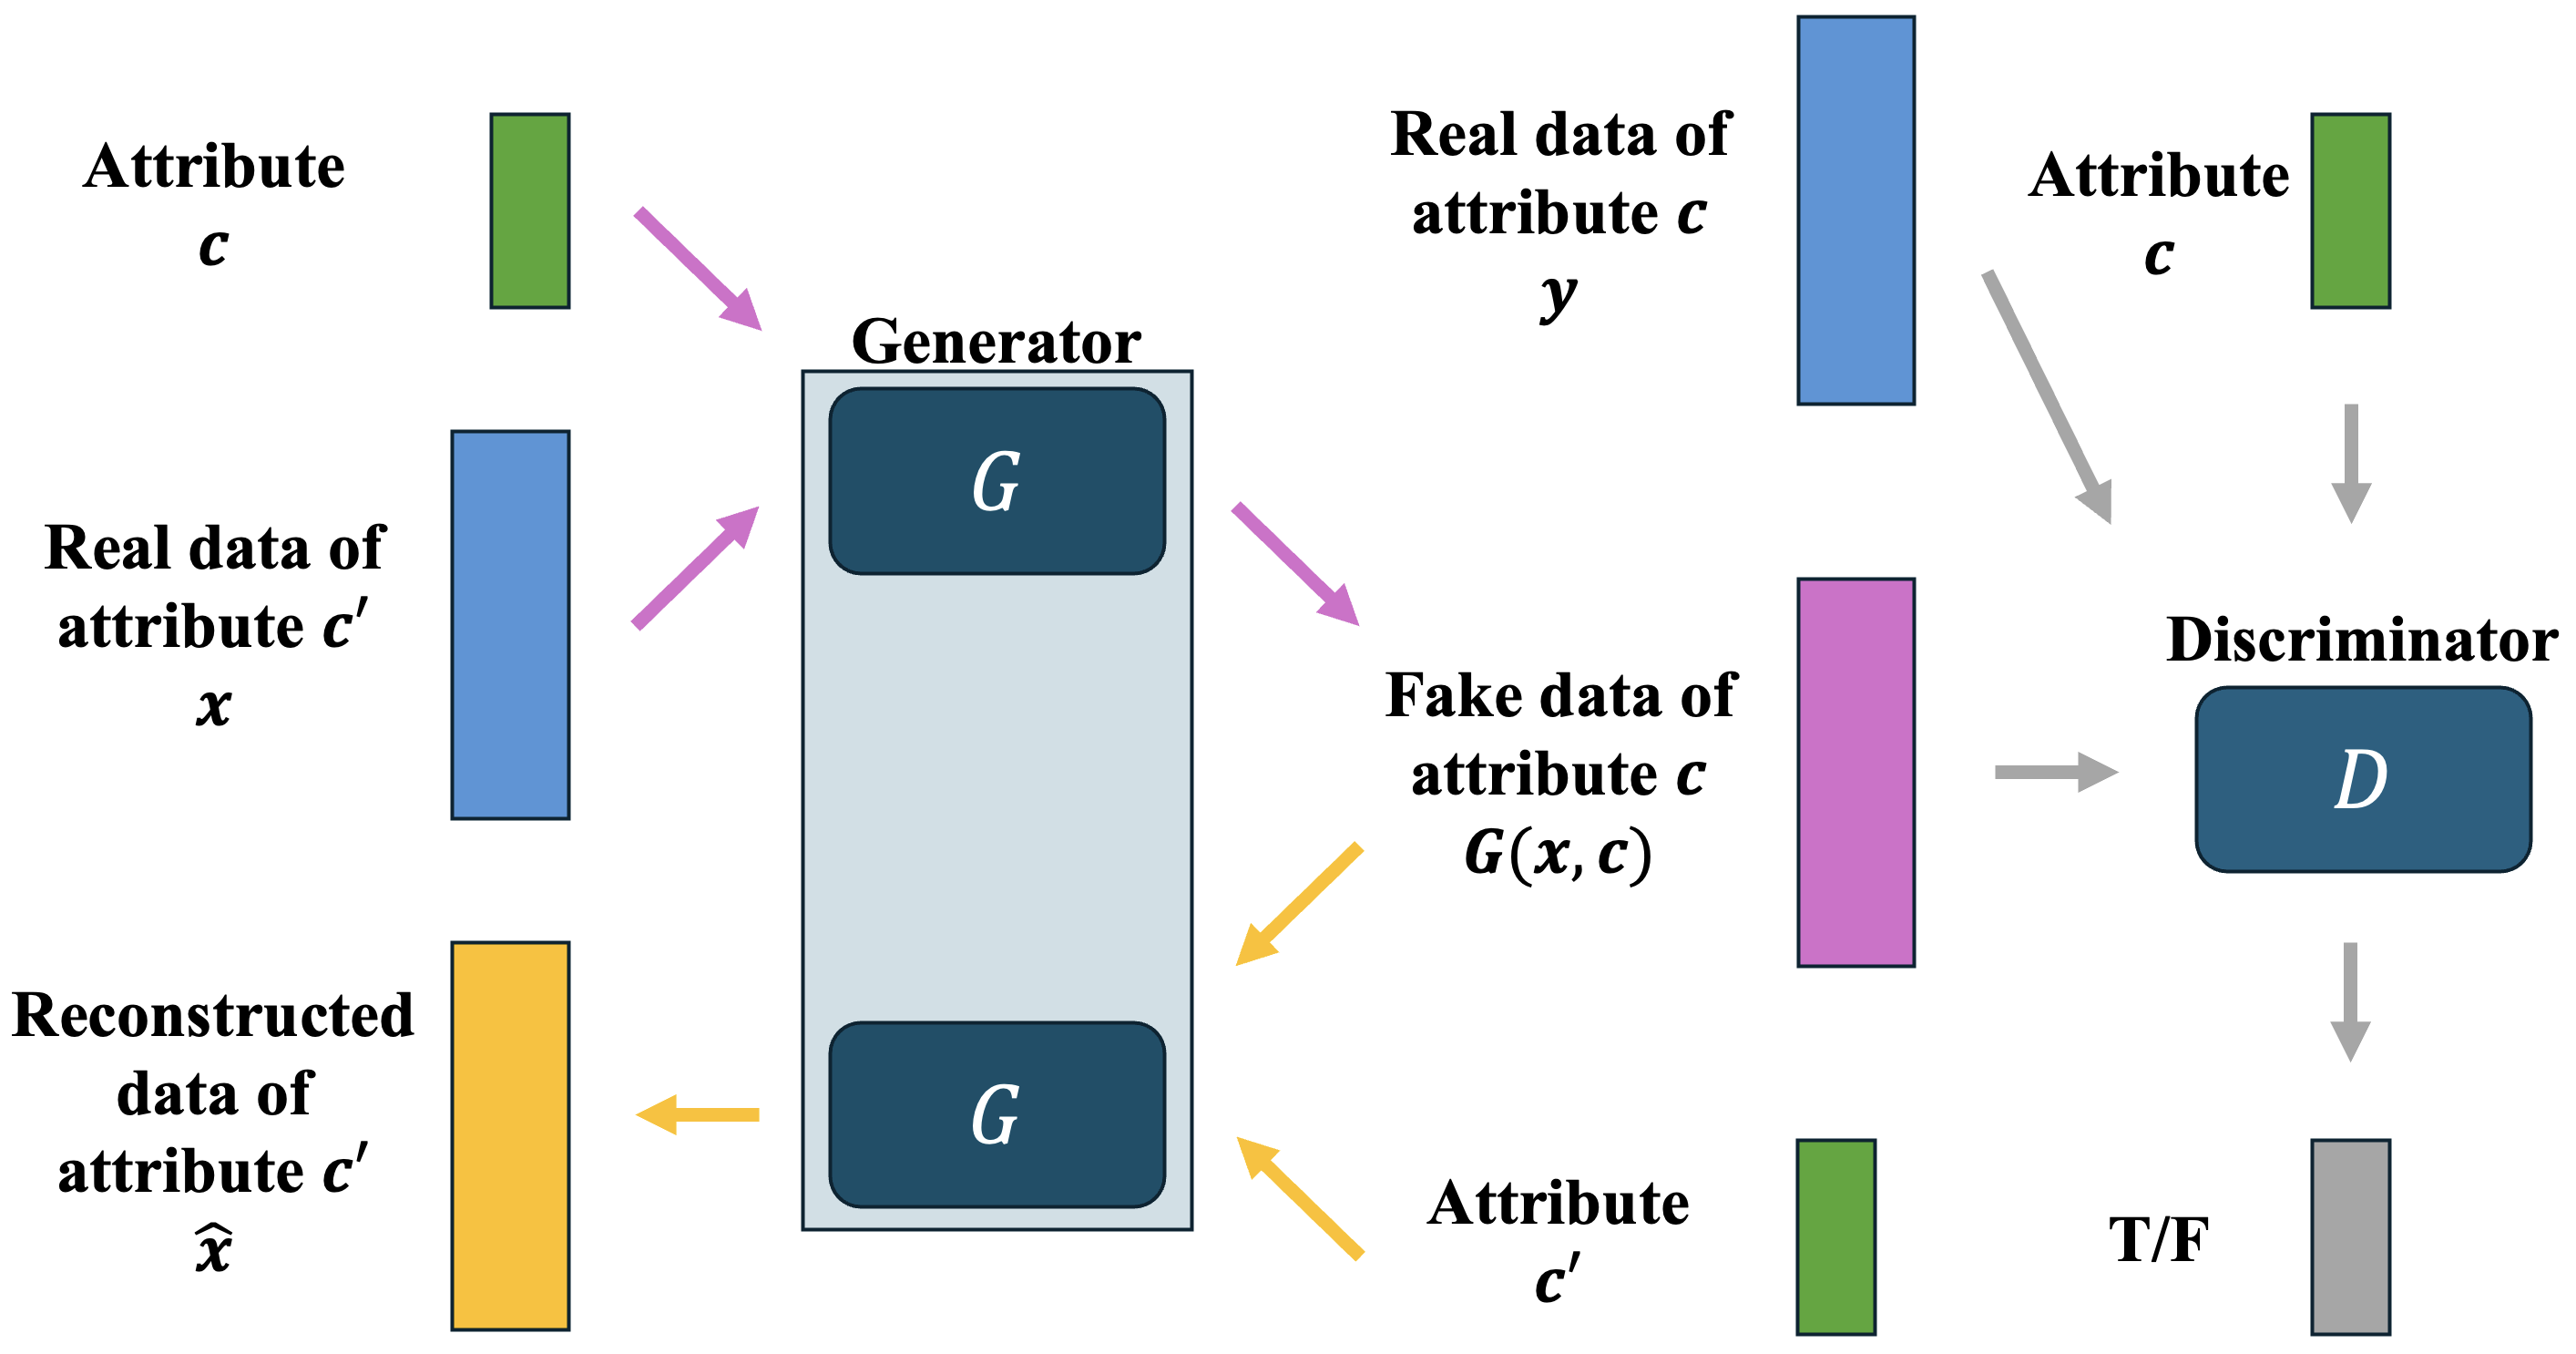
\includegraphics[scale=0.15]{img/undergraduate-thesis-arch.png}
        \end{figure}
    \end{block}
\end{frame}

\begin{frame}
    \frametitle{Projects}
    \begin{block}{3. Synthetic Data Generation using Conditional Normalizing Flows}
        \begin{itemize}
            \item Ability to replace original datasets and maintain same data distribution, and also highlight outliers for analysis.
            \item Built an B/S application to visualize results.
        \end{itemize}

        \begin{figure}[H]
            \centering
            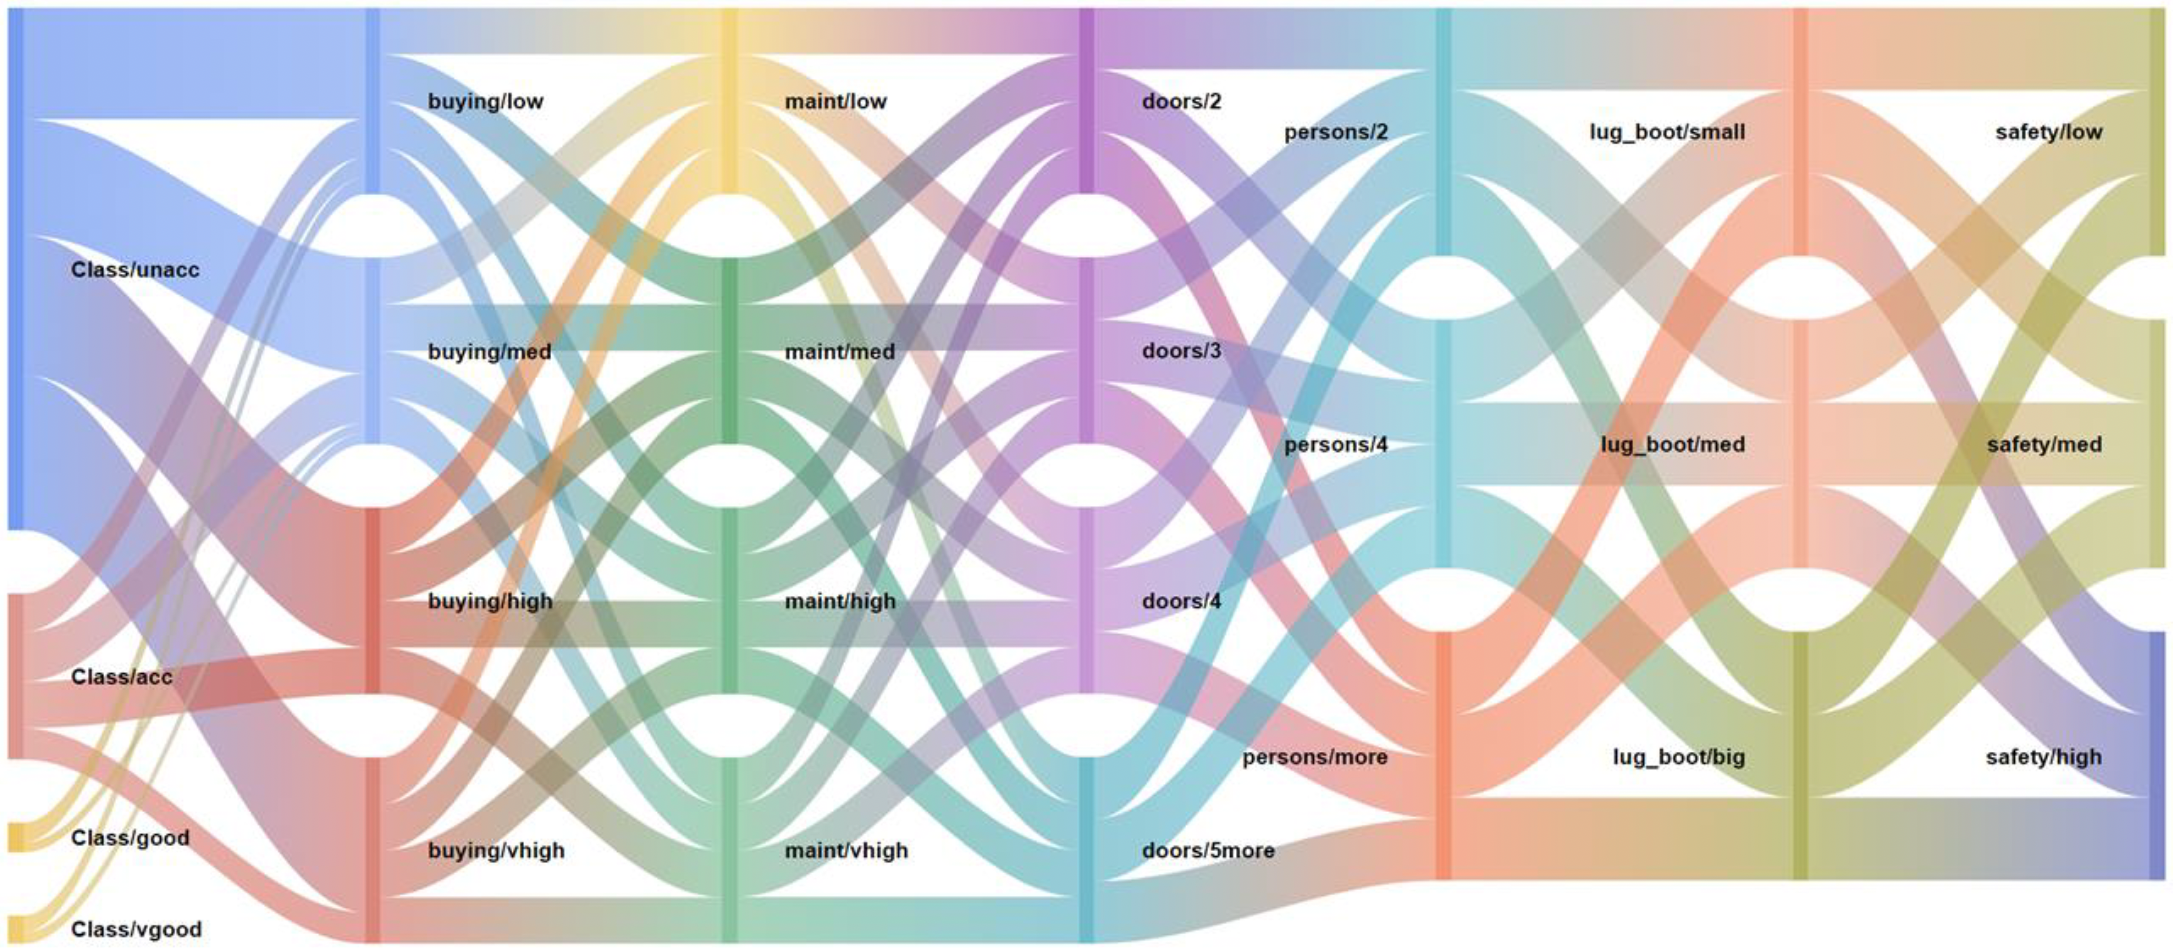
\includegraphics[scale=0.25]{img/cnf.png}
        \end{figure}
    \end{block}
\end{frame}

% TODO: Add architecture.
% \begin{frame}
%     \frametitle{Projects}
%     \begin{block}{4. (Master's Thesis, in progress) Floating image quality compensation algorithm technology}
%         \begin{itemize}
%             \item Simulated imaging process and enhanced the perceived image quality.
%             \item Ability to simulate on different devices with calculations performed only once per simulation.
%         \end{itemize}

%         \begin{figure}[H]
%             \centering
%             \includegraphics[scale=0.25]{img/floating-img-arch.png}
%         \end{figure}
%     \end{block}
% \end{frame}

%----------------------------------------------------------------------------------------
%	AWARDS SLIDES
%----------------------------------------------------------------------------------------

\section{Awards}
\begin{frame}
    \frametitle{Awards}
    \begin{block}{CCCC-Mobile Application Innovation Contest}
        First Prize \hfill 09 2018
    \end{block}
    \begin{block}{The 4th ”Internet+” Innovation and Entrepreneurship Competition}
        Gold Award \hfill 09 2018
    \end{block}
    \begin{block}{College Students’ Innovative Entrepreneurial Training Plan Program (SRTP)}
        Excellent \hfill 04 2018 – 05 2019
    \end{block}
\end{frame}

%----------------------------------------------------------------------------------------
%	EXPERIENCE SLIDES
%----------------------------------------------------------------------------------------

\section{Experience}
\begin{frame}
    \frametitle{Experience}
    \begin{block}{The University of British Columbia Vancouver Summer Program}
        Vancouver, Canada \hfill 07 2019 – 08 2019
        \begin{itemize}
            \item Included 2 courses, ”Algorithms and the World Wide Web” and ”Building Modern Web Applications”.
            \item Collaborated with my teammates to complete our projects as team leader.
        \end{itemize}
    \end{block}
\end{frame}

%----------------------------------------------------------------------------------------
%	SKILLS SLIDES
%----------------------------------------------------------------------------------------

\section{Skills}
\begin{frame}
    \frametitle{Skills}
    \begin{block}{Languages}
        Python, Java, C, JavaScript
    \end{block}
    \begin{block}{Technologies/Frameworks}
        PyTorch, Flask, Spring Boot, Vue.js, Git, SQL, MongoDB
    \end{block}
\end{frame}

\section{Thanks}
\begin{frame}
    \begin{center}
        \huge{\texttt{Thanks for your attention}} \\~\\
        \LARGE{Tzu-Chun, Oscar, Hsu} \\
        \vspace{8pt}
        \normalsize{
            Institute of Computer Science and Engineering, \\
            National Yang Ming Chiao Tung University (NYCU)} \\~\\
        \scriptsize{
            \href{tel:+886-987605719}{ \raisebox{-0.1\height}\faPhone\ \underline{+886-987605719} ~} 
            \href{mailto:vm3y3rmp40719@gmail.com}{\raisebox{-0.2\height}\faEnvelope\  \underline{vm3y3rmp40719@gmail.com}} \\~\\
            \href{https://www.linkedin.com/in/tzu-chun-hsu-ab4b3b188/}{\raisebox{-0.2\height}\faLinkedinSquare\ \underline{tzu-chun-hsu-ab4b3b188} ~}
            \href{https://github.com/Oscarshu0719}{\raisebox{-0.2\height}\faGithub\ \underline{Oscarshu0719}}
        }
    \end{center}
\end{frame}

\end{document}
